\documentclass[border=6pt]{standalone}
\usepackage{amsmath}
\usepackage{tikz}
\usetikzlibrary{arrows.meta}
\begin{document}
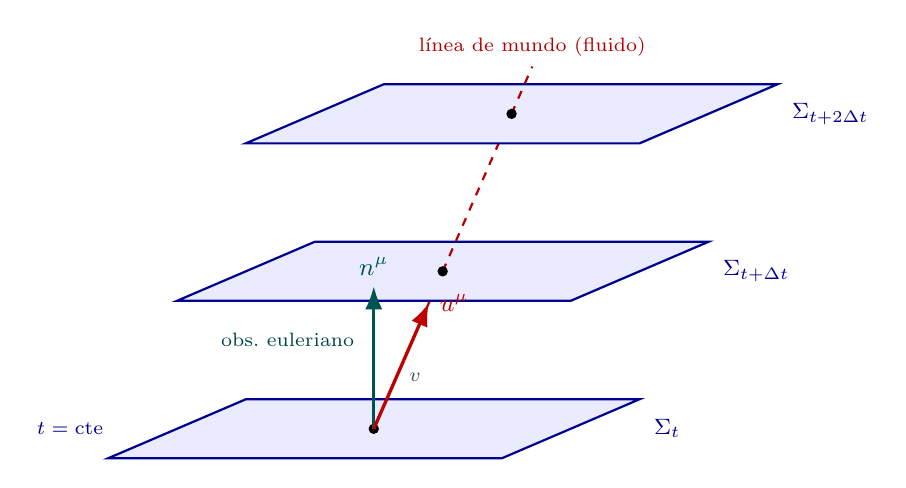
\begin{tikzpicture}[>=Latex,scale=1.25,
  plane/.style={thick,blue!55!black,fill=blue!8},
  wl/.style={thick,red!70!black,dashed}]

\def\s{0.7}\def\h{1.6}
% centros: P0=(0.3,0.3) P1=(1.0,1.9) P2=(1.7,3.5)
% Orden intercalado: cada plano se dibuja DESPUES del tramo de linea que viene
% de abajo, de modo que tapa la parte de la linea que queda detras (debajo del punto).

% --- Plano 0 (Sigma_t) ---
\draw[plane] (-2.4,0) -- (1.6,0) -- (3.0,0.6) -- (-1.0,0.6) -- cycle;
\node[blue!55!black,font=\footnotesize,anchor=west] at (3.05,0.3) {$\Sigma_{t}$};
\node[font=\scriptsize,blue!55!black,anchor=east] at (-2.35,0.3) {$t=\mathrm{cte}$};

% tramo de linea P0->P1 (delante del plano 0; su parte alta la tapara el plano 1)
\draw[wl] (0.3,0.3) -- (1.0,1.9);

% --- Plano 1 (Sigma_t+dt): tapa el tramo de linea que queda detras (bajo P1) ---
\draw[plane] ({-2.4+\s},{\h}) -- ({1.6+\s},{\h}) -- ({3.0+\s},{0.6+\h}) -- ({-1.0+\s},{0.6+\h}) -- cycle;
\node[blue!55!black,font=\footnotesize,anchor=west] at ({3.05+\s},{0.3+\h}) {$\Sigma_{t+\Delta t}$};

% tramo P1->P2 (delante del plano 1)
\draw[wl] (1.0,1.9) -- (1.7,3.5);

% --- Plano 2 (Sigma_t+2dt): tapa el tramo bajo P2 ---
\draw[plane] ({-2.4+2*\s},{2*\h}) -- ({1.6+2*\s},{2*\h}) -- ({3.0+2*\s},{0.6+2*\h}) -- ({-1.0+2*\s},{0.6+2*\h}) -- cycle;
\node[blue!55!black,font=\footnotesize,anchor=west] at ({3.05+2*\s},{0.3+2*\h}) {$\Sigma_{t+2\Delta t}$};

% tramo P2->arriba (delante del plano 2) con etiqueta
\draw[wl] (1.7,3.5) -- (1.91,3.98)
  node[above,font=\scriptsize,red!70!black,anchor=south] {l\'inea de mundo (fluido)};

% --- puntos: centro de cada plano (encima de todo) ---
\fill[black] (0.3,0.3) circle (1.5pt);
\fill[black] (1.0,1.9) circle (1.5pt);
\fill[black] (1.7,3.5) circle (1.5pt);

% --- vectores en el punto base (encima de todo) ---
\draw[->,very thick,teal!65!black] (0.3,0.3) -- ++(0,1.45) node[above,font=\small]{$n^{\mu}$};
\node[teal!55!black,font=\scriptsize,anchor=east] at (0.2,1.2) {obs.\ euleriano};
\draw[->,very thick,red!75!black] (0.3,0.3) -- ++(0.56,1.28) node[right,font=\small]{$u^{\mu}$};
\node[font=\scriptsize,black!70] at (0.72,0.82) {$v$};

\end{tikzpicture}
\end{document}
